\chapter{Gestión del riesgo y tamaño de posición}\label{cap:riesgo}

\begin{clave}[La regla más importante del curso]
Decide \textbf{cuánto puedes perder} antes de decidir cuánto puedes ganar. El tamaño de la posición se
calcula a partir del stop, no al revés.
\end{clave}

\section{Riesgo por operación y múltiplos de R}
Define $1R$ como el dinero que pierdes si salta el stop. Todo se mide en $R$: una operación que gana
$3R$ ganó tres veces lo arriesgado. Los profesionales arriesgan típicamente entre el 0,25~\% y el 1~\%
del capital por operación; rara vez más del 2~\%.

\section{Tamaño por stop}\label{sec:tamano}
Con capital $C$, riesgo $\rho$ (fracción), entrada $E$, stop $S$ y valor del punto $v$ (dinero por
unidad de precio y de tamaño):
\begin{equation}\label{eq:tamano}
N = \left\lfloor \frac{\rho\, C}{|E-S|\, v}\right\rfloor .
\end{equation}
\begin{table}[h]\centering\small
\begin{tabular}{lll}
\toprule
Mercado & Valor del punto $v$ & Función \\ \midrule
Acciones & 1 por acción & \py{risk.position\_size\_stop} \\
FX & valor del pip por lote $/$ tamaño del pip & \py{fx.pip\_value}, \py{fx.lots\_for\_risk} \\
Futuros & multiplicador del contrato (CL: 1000~\$) & \py{commodities.futures\_position\_size} \\
Stop por ATR & $|E-S| = k\cdot\text{ATR}$ & \py{risk.atr\_position\_size} \\
\bottomrule
\end{tabular}
\end{table}

\paragraph{Ejemplo.} Capital 50\,000~€, riesgo 0,5~\% (250~€), compra a 182,40 con stop en 176,90:
$N=\lfloor 250/5{,}50\rfloor = 45$ acciones. El nocional (8208~€) es solo el 16~\% del capital: el
riesgo lo fija el stop, no el nocional.
\begin{lstlisting}
python scripts/tamano_posicion.py accion --capital 50000 --riesgo 0.5 --entrada 182.4 --stop 176.9 --objetivo 195
\end{lstlisting}

\section{Volatility targeting}
En carteras y estrategias sistemáticas el tamaño se fija para que cada posición aporte una
volatilidad objetivo $\sigma^*$:
\begin{equation}
w_t = \min\!\left(\frac{\sigma^*}{\hat\sigma_t},\ L_{\max}\right),
\end{equation}
con $\hat\sigma_t$ estimada solo con datos hasta $t$ (\py{risk.vol\_target\_weight},
\py{backtest.vol\_targeted}). Reduce exposición cuando el mercado se agita, que es cuando suelen llegar
las pérdidas grandes.

\section{Kelly: cuánto arriesgar}
Si en cada apuesta ganas $b$ veces lo arriesgado con probabilidad $p$ y pierdes lo arriesgado con
probabilidad $1-p$, apostando una fracción $f$ del capital el crecimiento logarítmico esperado es
\begin{equation}
g(f) = p\ln(1+fb) + (1-p)\ln(1-f),
\end{equation}
que se maximiza en la \textbf{fracción de Kelly}
\begin{equation}\label{eq:kelly}
f^* = p - \frac{1-p}{b}\qquad\left(\text{continuo: } f^*=\frac{\mu}{\sigma^2}\right).
\end{equation}
\begin{figure}[h]\centering
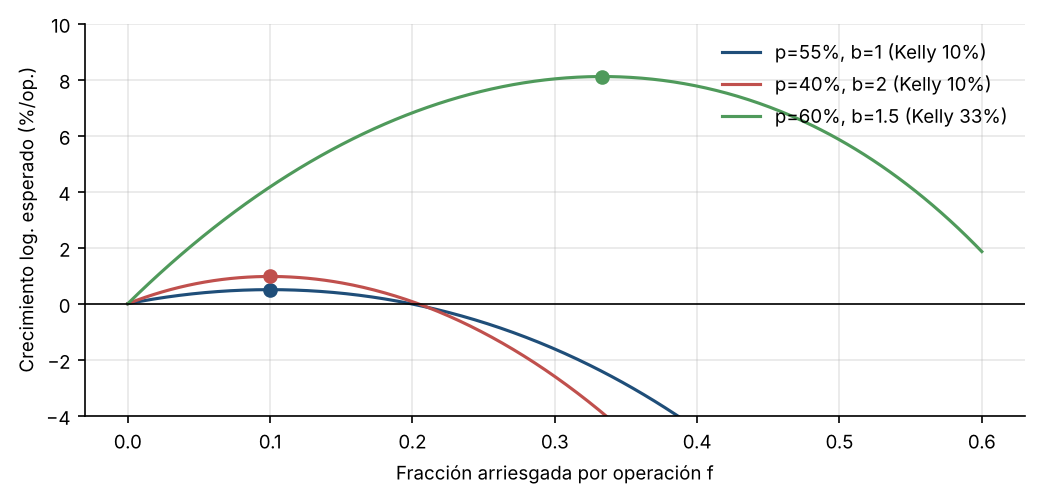
\includegraphics[width=0.85\textwidth]{f03_kelly}
\caption{Crecimiento esperado frente a la fracción arriesgada. Pasado Kelly el crecimiento cae y a
$2f^*$ es aproximadamente nulo: arriesgar de más destruye riqueza aunque la ventaja sea real.}
\label{fig:kelly}
\end{figure}

\begin{aviso}[Nunca uses Kelly completo]
$p$ y $b$ son estimaciones con mucho error. Sobrestimar la ventaja te lleva a la zona de la derecha de
la figura~\ref{fig:kelly}. Los profesionales usan entre $1/4$ y $1/2$ de Kelly, que sacrifica poco
crecimiento (con $f^*/2$ se obtiene en torno al 75~\% del crecimiento máximo) y reduce mucho la volatilidad.
\end{aviso}

\section{Riesgo de ruina y drawdown}
El drawdown es la caída desde el máximo previo, $DD_t = E_t/\max_{s\le t}E_s - 1$
(\py{risk.drawdown}). Recuperar una caída exige una subida mayor: tras perder un 50~\% hay que ganar
un 100~\%. La figura~\ref{fig:ruina} (Monte Carlo, \py{risk.risk\_of\_ruin\_mc}) muestra que la
probabilidad de sufrir un drawdown del 30~\% se dispara con el riesgo por operación, incluso con
ventaja real.
\begin{figure}[h]\centering
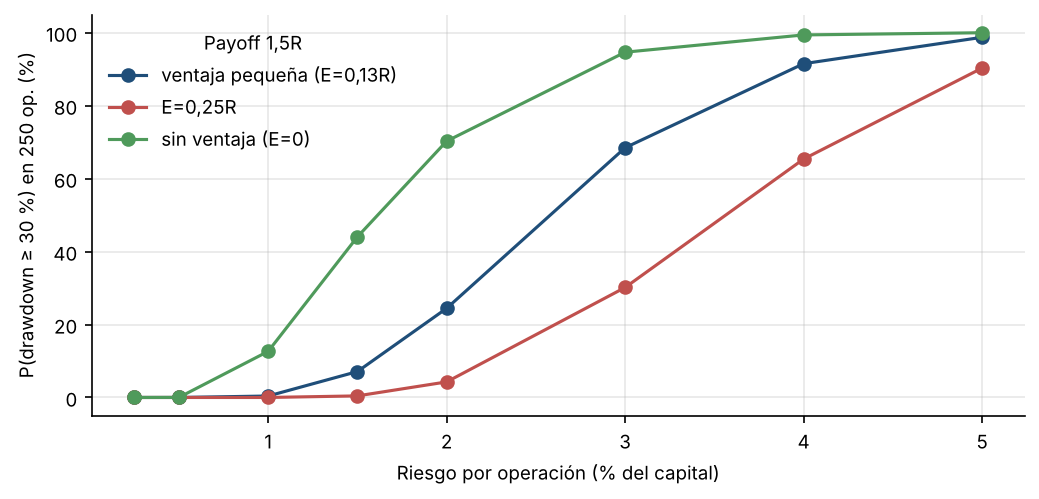
\includegraphics[width=0.85\textwidth]{f04_ruina}
\caption{Probabilidad de un drawdown $\ge 30~\%$ en 250 operaciones según el riesgo por operación.}
\label{fig:ruina}
\end{figure}

Con 10 pérdidas seguidas (algo frecuente con un 40~\% de acierto: $0{,}6^{10}\approx0{,}6~\%$ por
cada tramo de 10, pero en cientos de operaciones es casi seguro que ocurra alguna racha así), arriesgar
un 1~\% cuesta un 9,6~\%; arriesgar un 5~\% cuesta un 40~\%.

\section{Medidas de riesgo de cartera}
\paragraph{VaR y Expected Shortfall.} El VaR al nivel $\alpha$ es la pérdida que solo se supera con
probabilidad $1-\alpha$; el ES es la pérdida media \emph{cuando} se supera. Bajo normalidad
\begin{equation}
\text{VaR}_\alpha = -\mu - \sigma\,\Phi^{-1}(1-\alpha),\qquad
\text{ES}_\alpha = -\mu + \sigma\,\frac{\varphi(\Phi^{-1}(\alpha))}{1-\alpha}.
\end{equation}
Con $\mu=0$: VaR$_{99}=2{,}33\sigma$ y ES$_{97,5}=2{,}34\sigma$ (por eso Basilea usa ES al 97,5~\%).
La versión histórica usa los cuantiles empíricos (\py{risk.var\_historical}, \py{es\_historical}).

\paragraph{Contribuciones al riesgo.} Con pesos (o nocionales) $w$ y covarianza $\Sigma$,
$\sigma_p=\sqrt{w^\top\Sigma w}$ y la contribución de cada posición es
\begin{equation}
RC_i = \frac{w_i (\Sigma w)_i}{\sigma_p},\qquad \sum_i RC_i = \sigma_p .
\end{equation}
Una posición pequeña pero muy correlacionada con el resto puede dominar el riesgo.
\py{scripts/informe\_riesgo.py} muestra la tabla de contribuciones, VaR/ES y un estrés común.

\section{Límites de una mesa profesional}
\begin{itemize}
\item \textbf{Pérdida diaria máxima} (p.~ej. 2--3~\% del capital o 3R): al tocarla, se deja de operar ese día.
\item \textbf{Drawdown máximo} (p.~ej. 10~\%): al tocarlo, se reduce el tamaño a la mitad hasta recuperar.
\item \textbf{Riesgo abierto total}: suma de las distancias a los stops $\le$ 4--6~\% del capital.
\item \textbf{Concentración}: límites por activo, sector, divisa y factor.
\item \textbf{Apalancamiento bruto} y \textbf{liquidez}: no tener más de un 10--20~\% del volumen diario.
\end{itemize}

\begin{ejercicios}
\begin{enumerate}
\item Con $p=0{,}45$ y $b=2$, calcula Kelly y medio Kelly. Comprueba con \py{risk.growth\_rate} que medio Kelly da aproximadamente el 75~\% del crecimiento.
\item Tu sistema tiene un 35~\% de acierto. ¿Qué probabilidad hay de 8 pérdidas consecutivas en una secuencia concreta de 8? Simula cuántas rachas así aparecen en 500 operaciones.
\item Ejecuta \py{scripts/informe\_riesgo.py} y explica por qué el VaR histórico al 99~\% difiere del normal.
\end{enumerate}
\end{ejercicios}
